\section{Practical experiment}
In order to validate our system we have developed a practical experiment based on one of the conceptual experiments described in \autoref{chap:sys-arch}.

The base idea of the practical experiment is to control the velocity of the motor using both the local control on the slave device and the remote control concept, where the RTE network is intercalated on the control loop, using a few different configuration values for the network cycle time.

During the local control mode, only the set-point values of the velocity curve will be transmitted over the RTE network, so the expected behaviour is for the network cycle time to barely affect the performance of the velocity control loop.
The expected result is for the actual velocity of the motor to follow the expected curve with, at most, a small increment to the response time of the process, with the same order of magnitude of the chosen network cycle time.

On the other hand, the remote control mode will have the master node of the RTE network performing the necessary computations and the slave node device will act as a simple networked I/O interface for the system.
This way, the control loop will traverse the slave device and the RTE network before being closed on the master device.
This mode of operation is expected to have a significant impact on the performance of the control loop because the network cycle time will influence the communication delay in both directions.
Not only the plant feedback value will be delayed on its way from the slave device to the master device but also the output value will be delayed on the opposite direction.
This delay is expected to heavily impact the performance of the velocity control loop and we expect to obtain either a system with much slower dynamics or, under an extreme condition of network cycle time, a system that might not be controllable.

% Velocity curve definition
For this experiment we have defined a velocity curve comprised of six different stages.
Each stage will set the velocity to a single final value, making the set-point preview curve have five step transitions.
The graph shown in \autoref{fig:velocity-curve} has been generated to help visualise the curve.

\begin{figure}[htp]
	\centering
	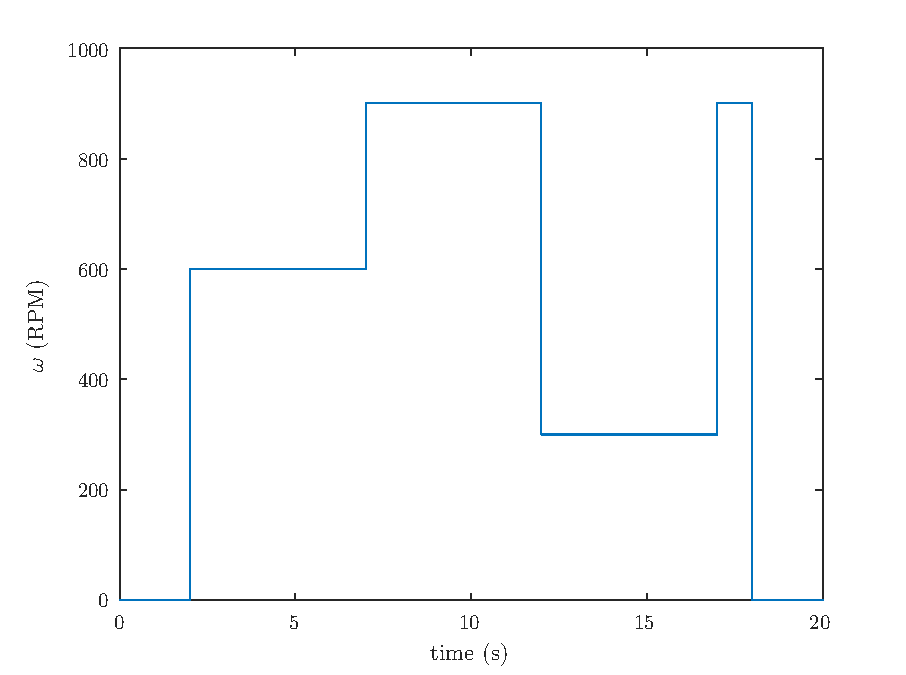
\includegraphics[width=0.8\linewidth]{velocity-curve.PNG}
	\caption{Preview of the defined velocity curve}
	\label{fig:velocity-curve}
\end{figure}

We expect this velocity curve to provide us with enough variability in both the time and controlled variable domains in order to properly evaluate the system performance in all test cases.

% Network cycle times to use
% `- with a task of 10ms maybe use 5ms, 10ms and 20ms of network cycle time?
When creating a new CODESYS project, the main task is configured by default with a cycle time of 20ms, but because we intend to implement motion control, we will use a cycle time of 10ms.
This period will also be configured on the slave device so that value updates occur at the same speed as the processing on the master device.
We will perform three tests with each control mode using three different network cycle periods: 5ms, 10ms and 20ms, which are half, full and double of the processing period, respectively.
This effectively means we will present six test cases and compare the performance between local/remote control mode pairs for each network cycle period.

\subsection{Master node implementation}
In the particular case of this experiment, the master node device is implemented on a generic desktop PC.
It has been programmed using the CODESYS platform and is running on top of Windows 10\texttrademark{}.

Because this OS doesn't officially provide support for running real-time applications, the hardware specifications of the underlying PC shouldn't really influence the outcome of the experiment, as the OS is expected to have a bigger influence through its process management.
With that being sad, the master node device is a home-built desktop computer comprised of an AMD Ryzen\texttrademark{} 5 1600 CPU \cite{hdw:ryzen5-1600}, an MSI X470 Gaming Plus \cite{hdw:msi-x470} motherboard with 2x8GB dual-channel Kingston HyperX Fury DDR4 RAM (16GB total) \cite{hdw:hyperx-fury-8gb-ddr4-2400} running at 2400MHz, a 500GB Samsung 970 Evo Plus NVMe\textregistered{} M.2 SSD \cite{hdw:970evo-plus-ssd} hard drive, a Gigabyte GeForce\textregistered{} GTX 1650 Super\texttrademark{} OC 4G \cite{hdw:gigabyte-1650-super-oc} graphics card (NVIDIA) and it is powered by an Aerocool KCAS 500W PSU \cite{hdw:kcas-500w}.

The CODESYS platform was used to create a single program on the master node that sends the velocity set-points of the predefined velocity curve over the RTE network to the slave device, receives the plant feedback values from the RTE network, performs the necessary computations for the control loop and sends the the computed plant output value to the slave node, also through the RTE network.
Because the slave device software ignores the output value arriving on the RTE network interface when it is configured for local control, the same software can be used on the master node for both experiences with local and remote control modes.
Furthermore, this approach makes sure all data to be exported is present on the slave device in both operation modes.

The CODESYS platform includes support to create a Software PLC (SoftPLC) that runs on the desktop PC.
The program is then downloaded to it, as if it was a traditional PLC.
The master device program was implemented in four different Program Organisation Unit (POU) implemented in three different IEC 61131-3 programming languages: 
\begin{itemize}
	\item Structured Text (ST) was used in two POUs that perform data type manipulations;
	\item Sequential Function Chart (SFC) was used to program a simple state machine;
	\item Lastly, Function Block Diagram (FBD) was used to map different variables into and out of a PID computation block.
\end{itemize}

The EtherCAT cyclic process data is statically defined as bytes.
As such, two POUs were programmed in order to convert bytes into \verb|word| (2-byte integer numbers) or \verb|real| (floating point variables) variables, as necessary.
One POU will agregate the input data arriving from the slave device as bytes into global variables and the second POU will split the output global variables into bytes.
